
\documentclass[11pt]{article}

% Set the margins to be something normal.
\usepackage[margin=1in]{geometry}

% Fun lists!
\usepackage{enumitem}
\usepackage{textcomp}
\setitemize{label=\textrightarrow, itemsep=0pt}

% Math symbols.
\usepackage{amsmath, amssymb, amsfonts}
\usepackage{tikz, xcolor}
\usepackage{tikz-3dplot}
\usetikzlibrary{arrows}

% No indents.
\setlength\parindent{0pt}

% Nice fonts :)
\usepackage{tgschola}

\begin{document}
	{
		\centering
		\huge{Week 2 Recitation Problems} \\
		\Large{MATH:114, Recitations 309 and 310} \\
	}
	
	\vspace{3em}
	
	1. Suppose $f(x)=(x-1)^2$ and $g(x)=2(x-1)+3$. Plot these functions, and shade the region enclosed by them. Where do the curves intersect? What is the area of the enclosed region?
	
	\vspace{20em}
	
	2. Take the region you drew and spin it all the way around the $x$-axis. This is called a \textit{solid of revolution}, and it lives in \rule{1em}{1pt}-dimensional space. Now, draw cross-sections of the solid along the
		\begin{enumerate}[label=(\alph*)]
			\item $xy$ plane that intersects the $z$-axis at the origin.
			\item $yz$ plane that intersects the $x$-axis at $x=3$
			\item $xz$ plane that intersects the $y$-axis at $y=1$.
		\end{enumerate}
		\vspace{2em}
		
		\begin{center}
			\scalebox{.75}{
				\tdplotsetmaincoords{0}{0}
				
				% (a)
				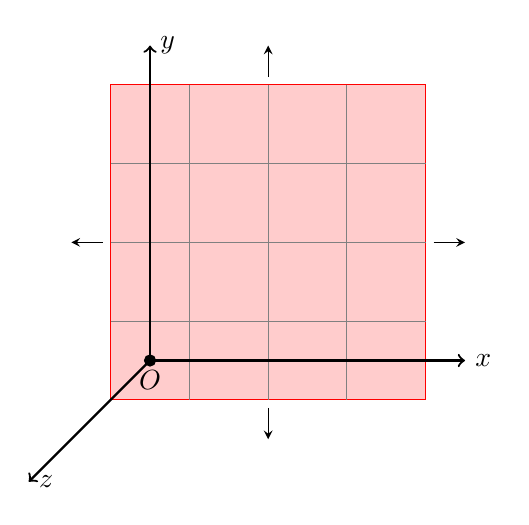
\begin{tikzpicture}
					[
						axis/.style={->,black,thick}
					]
					
					% Draw XY plane.
					\filldraw[
				        draw=red,%
				        fill=red!20,%
				    ]          (-1/2,-1/2,0)
				            -- (3.5,-1/2,0)
				            -- (3.5,3.5,0)
				            -- (-1/2,3.5,0)
				            -- cycle;
				            
				    % Draw points.
				    \filldraw[black] (0,0) circle (2pt) node[anchor=north]{$O$};
				    
				    % Draw grid.
				    \draw[gray, thin] (-1/2,1/2,0) -- (3.5,1/2,0);
				    \draw[gray, thin] (-1/2,3/2,0) -- (3.5,3/2,0);
				    \draw[gray, thin] (-1/2,5/2,0) -- (3.5,5/2,0);
				    \draw[gray, thin] (1/2,7/2,0) -- (1/2,-1/2,0);
				    \draw[gray, thin] (3/2,7/2,0) -- (3/2,-1/2,0);
				    \draw[gray, thin] (5/2,7/2,0) -- (5/2,-1/2,0);
				    
				    % Draw arrows to indicate the plane goes on forever.
				    \draw [-stealth](3.6, 1.5) -- (4, 1.5);
				    \draw [-stealth](3/2, -.6) -- (3/2, -1);
				    \draw [-stealth](-.6, 1.5) -- (-1, 1.5);
				    \draw [-stealth](3/2, 3.6) -- (3/2, 4);
				            
				    % Plot axes.
					\draw[axis] (0,0,0) -- (4,0,0) node[anchor=west]{$x$};
					\draw[axis] (0,0,0) -- (0,4,0) node[anchor=west]{$y$};
					\draw[axis] (0,0,0) -- (0,0,4) node[anchor=west]{$z$};
				\end{tikzpicture}\hspace{3em}
				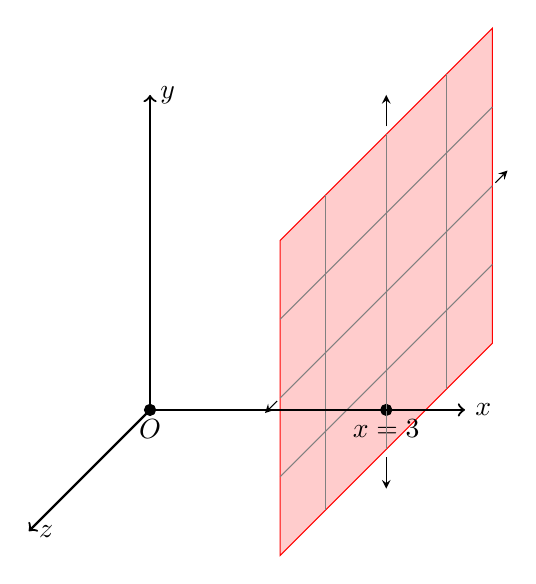
\begin{tikzpicture}
					[
						axis/.style={->,black,thick}
					]
					
					% Draw XY plane.
					\filldraw[
				        draw=red,%
				        fill=red!20,%
				    ]          (3,-1/2,3.5)
				            -- (3,-1/2,-3.5)
				            -- (3,3.5,-3.5)
				            -- (3,3.5,3.5)
				            -- cycle;
				            
				    % Draw points.
				    \filldraw[black] (0,0) circle (2pt) node[anchor=north]{$O$};
				    \filldraw[black] (3,0) circle (2pt) node[anchor=north]{$x=3$};
				    
				    % Draw grid.
				    \draw[gray, thin] (3,1/2,-3.5) -- (3,1/2,3.5);
				    \draw[gray, thin] (3,3/2,-3.5) -- (3,3/2,3.5);
				    \draw[gray, thin] (3,5/2,-3.5) -- (3,5/2,3.5);
				    \draw[gray, thin] (3,7/2,2) -- (3,-1/2,2);
				    \draw[gray, thin] (3,7/2,0) -- (3,-1/2,0);
				    \draw[gray, thin] (3,7/2,-2) -- (3,-1/2,-2);
				    
				    % Draw arrows to indicate the plane goes on forever.
				    \draw [-stealth](3,1.5,3.6) -- (3,1.5,4);
				    \draw [-stealth](3,1.5,-3.6) -- (3,1.5,-4);
				    \draw [-stealth](3,3.6,0) -- (3,4,0);
				    \draw [-stealth](3,-.6,0) -- (3,-1,0);
				            
				    % Plot axes.
					\draw[axis] (0,0,0) -- (4,0,0) node[anchor=west]{$x$};
					\draw[axis] (0,0,0) -- (0,4,0) node[anchor=west]{$y$};
					\draw[axis] (0,0,0) -- (0,0,4) node[anchor=west]{$z$};
				\end{tikzpicture}\hspace{3em}
				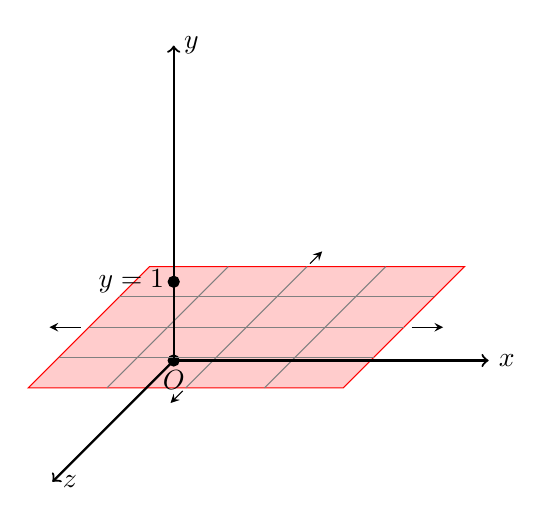
\begin{tikzpicture}
					[
						axis/.style={->,black,thick}
					]
					
					% Draw XY plane.
					\filldraw[
				        draw=red,%
				        fill=red!20,%
				    ]          (-1/2,1,3.5)
				            -- (3.5,1,3.5)
				            -- (3.5,1,-1/2)
				            -- (-1/2,1,-1/2)
				            -- cycle;
				            
				    % Draw points.
				    \filldraw[black] (0,0) circle (2pt) node[anchor=north]{$O$};
				    \filldraw[black] (0,1) circle (2pt) node[anchor=east]{$y=1$};
				    
				    % Draw arrows to indicate the plane goes on forever.
				    \draw [-stealth](1.5, 1, 3.6) -- (1.5, 1, 4);
				    \draw [-stealth](1.5, 1, -.6) -- (1.5, 1, -1);
				    \draw [-stealth](-.6, 1, 3/2) -- (-1, 1, 3/2);
				    \draw [-stealth](3.6, 1, 3/2) -- (4, 1, 3/2);
				    
				    % Draw grid.
				    \draw[gray, thin] (-1/2,1,5/2) -- (3.5,1,5/2);
				    \draw[gray, thin] (-1/2,1,3/2) -- (3.5,1,3/2);
				    \draw[gray, thin] (-1/2,1,1/2) -- (3.5,1,1/2);
				    \draw[gray, thin] (1/2,1,3.5) -- (1/2,1,-1/2);
				    \draw[gray, thin] (3/2,1,3.5) -- (3/2,1,-1/2);
				    \draw[gray, thin] (5/2,1,3.5) -- (5/2,1,-1/2);
				            
				    % Plot axes.
					\draw[axis] (0,0,0) -- (4,0,0) node[anchor=west]{$x$};
					\draw[axis] (0,0,0) -- (0,4,0) node[anchor=west]{$y$};
					\draw[axis] (0,0,0) -- (0,0,4) node[anchor=west]{$z$};
				\end{tikzpicture}
			}
		\end{center}
		
		\newpage
		3. Write a formula for the area of each cross-section (hint: one is too hard, and two are familiar geometric ones). If we ``shift'' our intersection plane along the length of the solid, finding the area of each cross-section, what is the \textit{sum} of these areas?
		
		\vspace{0.4\paperheight}
		
		4. Choose an intersection plane. Write an integral that represents the sum of all the cross-sectional areas we get by shifting the plane along the solid.


\end{document}
